\documentclass[11pt]{article}

\usepackage{amsmath,amssymb}
\usepackage{tikz}
\usetikzlibrary{arrows.meta,positioning,fit,calc}

\begin{document}

\begin{figure}[t]
\centering

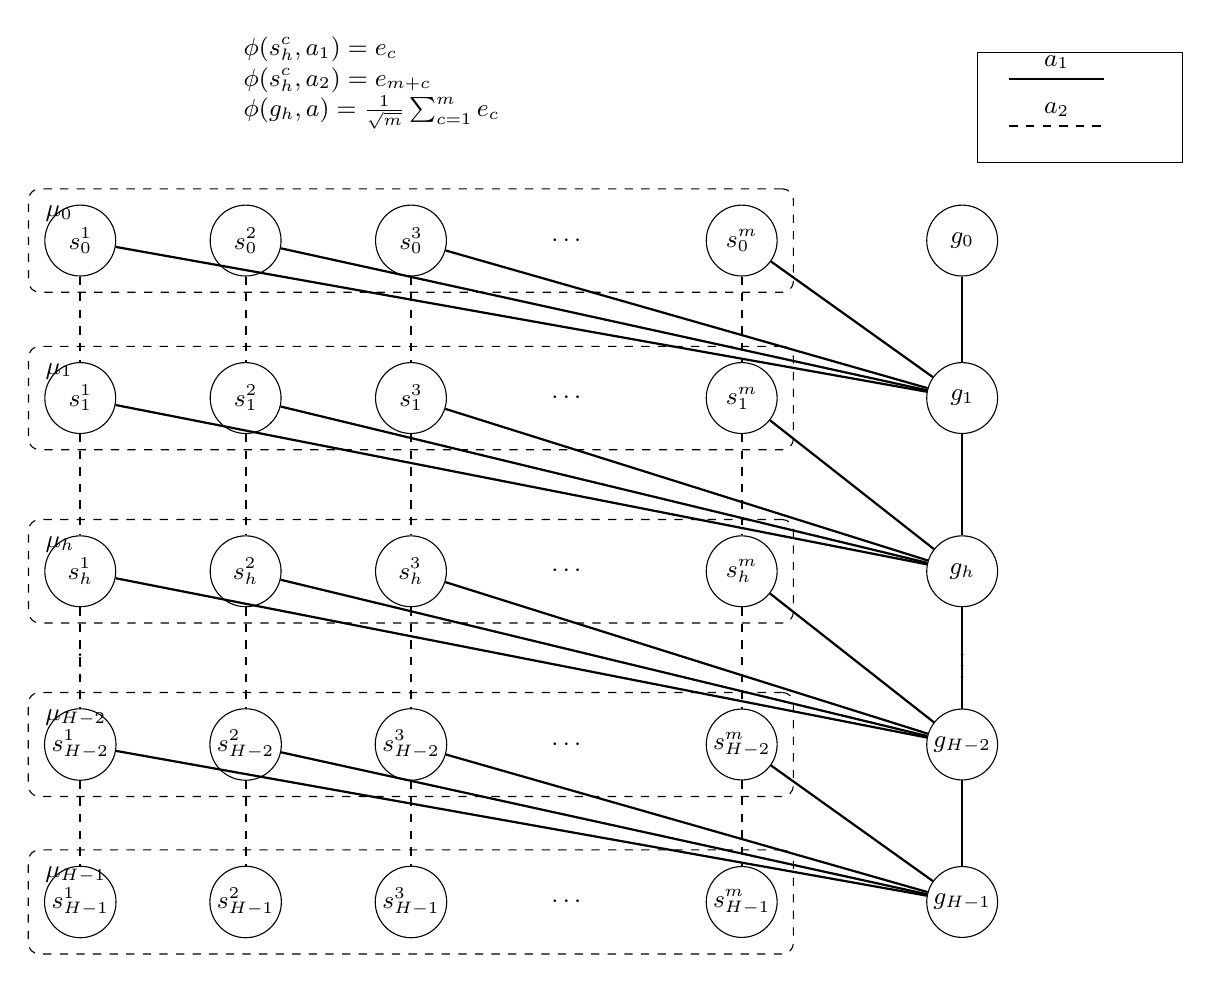
\begin{tikzpicture}[
  >=Latex,
  font=\small,
  state/.style={circle,draw,minimum size=9mm,inner sep=1pt},
  obsbox/.style={draw,dashed,rounded corners,inner sep=2mm},
  aone/.style={thick},
  atwo/.style={thick,dashed}
]

% -------------------------
% Geometry (no digits in macro names)
% -------------------------
\def\xOne{0}
\def\xTwo{2.1}
\def\xThree{4.2}
\def\xDots{6.2}
\def\xLast{8.4}
\def\xAgg{11.2}

\def\yRowZero{0}
\def\yRowOne{-2.0}
\def\yRowMid{-4.2}
\def\yRowHm{-6.4}
\def\yRowH{-8.4}

% -------------------------
% Top text: features + legend
% -------------------------
\node[align=left] at (3.7,2.0) {$\phi(s_h^c,a_1)=e_c$\\
$\phi(s_h^c,a_2)=e_{m+c}$\\
$\phi(g_h,a)=\frac{1}{\sqrt m}\sum_{c=1}^m e_c$};

% Legend box
\node[draw,minimum width=2.6cm,minimum height=1.4cm,anchor=north east] (leg) at (\xAgg+2.8,2.4) {};
\draw[aone] ([xshift=-2.2cm,yshift=-0.35cm]leg.north east) -- ++(1.2,0) node[midway,above] {$a_1$};
\draw[atwo] ([xshift=-2.2cm,yshift=-0.95cm]leg.north east) -- ++(1.2,0) node[midway,above] {$a_2$};

% -------------------------
% Nodes
% -------------------------

% Row h=0
\node[state] (s0-1) at (\xOne,\yRowZero) {$s_0^{1}$};
\node[state] (s0-2) at (\xTwo,\yRowZero) {$s_0^{2}$};
\node[state] (s0-3) at (\xThree,\yRowZero) {$s_0^{3}$};
\node        (s0-d) at (\xDots,\yRowZero) {$\cdots$};
\node[state] (s0-m) at (\xLast,\yRowZero) {$s_0^{m}$};
\node[state] (g0)   at (\xAgg,\yRowZero) {$g_0$};

% Row h=1
\node[state] (s1-1) at (\xOne,\yRowOne) {$s_1^{1}$};
\node[state] (s1-2) at (\xTwo,\yRowOne) {$s_1^{2}$};
\node[state] (s1-3) at (\xThree,\yRowOne) {$s_1^{3}$};
\node        (s1-d) at (\xDots,\yRowOne) {$\cdots$};
\node[state] (s1-m) at (\xLast,\yRowOne) {$s_1^{m}$};
\node[state] (g1)   at (\xAgg,\yRowOne) {$g_1$};

% Row h (generic)
\node[state] (sh-1) at (\xOne,\yRowMid) {$s_h^{1}$};
\node[state] (sh-2) at (\xTwo,\yRowMid) {$s_h^{2}$};
\node[state] (sh-3) at (\xThree,\yRowMid) {$s_h^{3}$};
\node        (sh-d) at (\xDots,\yRowMid) {$\cdots$};
\node[state] (sh-m) at (\xLast,\yRowMid) {$s_h^{m}$};
\node[state] (gh)   at (\xAgg,\yRowMid) {$g_h$};

% Row H-2
\node[state] (sHm-1) at (\xOne,\yRowHm) {$s_{H-2}^{1}$};
\node[state] (sHm-2) at (\xTwo,\yRowHm) {$s_{H-2}^{2}$};
\node[state] (sHm-3) at (\xThree,\yRowHm) {$s_{H-2}^{3}$};
\node         (sHm-d) at (\xDots,\yRowHm) {$\cdots$};
\node[state] (sHm-m) at (\xLast,\yRowHm) {$s_{H-2}^{m}$};
\node[state] (gHm)   at (\xAgg,\yRowHm) {$g_{H-2}$};

% Row H-1
\node[state] (sH-1) at (\xOne,\yRowH) {$s_{H-1}^{1}$};
\node[state] (sH-2) at (\xTwo,\yRowH) {$s_{H-1}^{2}$};
\node[state] (sH-3) at (\xThree,\yRowH) {$s_{H-1}^{3}$};
\node        (sH-d) at (\xDots,\yRowH) {$\cdots$};
\node[state] (sH-m) at (\xLast,\yRowH) {$s_{H-1}^{m}$};
\node[state] (gH)   at (\xAgg,\yRowH) {$g_{H-1}$};

% -------------------------
% Data support boxes: only observed states
% -------------------------
\node[obsbox,fit=(s0-1)(s0-m)] (box0) {};
\node[obsbox,fit=(s1-1)(s1-m)] (box1) {};
\node[obsbox,fit=(sh-1)(sh-m)] (boxh) {};
\node[obsbox,fit=(sHm-1)(sHm-m)] (boxHm) {};
\node[obsbox,fit=(sH-1)(sH-m)] (boxH) {};

\node[anchor=north west] at ([xshift=1mm,yshift=-1mm]box0.north west) {$\mu_0$};
\node[anchor=north west] at ([xshift=1mm,yshift=-1mm]box1.north west) {$\mu_1$};
\node[anchor=north west] at ([xshift=1mm,yshift=-1mm]boxh.north west) {$\mu_h$};
\node[anchor=north west] at ([xshift=1mm,yshift=-1mm]boxHm.north west) {$\mu_{H-2}$};
\node[anchor=north west] at ([xshift=1mm,yshift=-1mm]boxH.north west) {$\mu_{H-1}$};

% -------------------------
% Transitions: a2 dashed (stay observed), a1 solid (jump to aggregator)
% -------------------------

% a2 edges (vertical, observed chain)
\foreach \u/\v in {s0-1/s1-1,s0-2/s1-2,s0-3/s1-3,s0-m/s1-m,
                  s1-1/sh-1,s1-2/sh-2,s1-3/sh-3,s1-m/sh-m,
                  sh-1/sHm-1,sh-2/sHm-2,sh-3/sHm-3,sh-m/sHm-m,
                  sHm-1/sH-1,sHm-2/sH-2,sHm-3/sH-3,sHm-m/sH-m} {
  \draw[atwo] (\u) -- (\v);
}

% a1 edges (diagonal to aggregator at next layer)
\foreach \u/\v in {s0-1/g1,s0-2/g1,s0-3/g1,s0-m/g1,
                  s1-1/gh,s1-2/gh,s1-3/gh,s1-m/gh,
                  sh-1/gHm,sh-2/gHm,sh-3/gHm,sh-m/gHm,
                  sHm-1/gH,sHm-2/gH,sHm-3/gH,sHm-m/gH} {
  \draw[aone] (\u) -- (\v);
}

% aggregator chain
\draw[aone] (g0) -- (g1);
\draw[aone] (g1) -- (gh);
\draw[aone] (gh) -- (gHm);
\draw[aone] (gHm) -- (gH);

% dots
\node at (\xAgg,{-5.3}) {$\vdots$};
\node at (\xOne,{-5.3}) {$\vdots$};

\end{tikzpicture}

\caption{\textbf{Offline policy-evaluation hard instance (schematic).}
Each layer $h$ has $m$ ``observed'' states $\{s_h^c\}_{c=1}^m$ (boxed: support of $\mu_h$)
and one ``aggregator'' state $g_h$ (not in the support of $\mu_h$).
Action $a_2$ (dashed) keeps the trajectory in the observed chain $s_h^c\to s_{h+1}^c$,
while $a_1$ (solid) jumps to the aggregator chain $s_h^c\to g_{h+1}$.}
\label{fig:offline_pe_hard_instance_clean}
\end{figure}

\end{document}
